\begin{Exercise}[title={Stack},difficulty=5]
\label{ex:stack}
\Question \label{ex:stack q1} Create a simple stack which can hold a
fixed amount of \key{int}s. It does not have to grow beyond this limit.
Define both a \func{push} -- put something on the stack -- and a \func{pop} 
-- retrieve something fro the stack -- function. The stack should be
a FIFO (last in, first out) stack.

\begin{center}
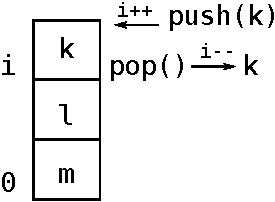
\includegraphics[scale=0.90]{fig/stack.pdf}
\label{fig:stack}
\end{center}

\Question \label{ex:stack q2} Bonus. Write a \func{String} method which 
converts the stack to a string representation.  This way you can print the stack using:
\lstinline{fmt.Printf("My stack %v\n", stack)}

\noindent{}The stack in the figure could be represented as:
\begin{alltt}
[0:m] [1:l] [2:k]
\end{alltt}
\end{Exercise}

\begin{Answer}

\Question 
%%\subsection*{Define our type} maybe nice to do this
First we define a new type that represents a stack; we need an
array (to hold the keys) and an index, which points to the last element.
Our small stack only holds 10 elements.

\begin{lstlisting}
type stack struct { |\coderemark{\emph{stack} is not exported}|
    i    int 
    data [10]int
}
\end{lstlisting}

Next we need the \func{push} and \func{pop} functions to actually
use the damn thing. \emph{First we show the \textbf{WRONG} solution!}
In Go data passed to functions is \emph{passed-by-value} meaning a copy
is created and given to the function. The first stab for the function
\func{push} could be:

\begin{lstlisting}
func (s stack) push(k int) (ok bool) {
	if s.i+1 > 9 {
		return false
	}
	s.data[s.i] = k
	s.i++
	return true
}
\end{lstlisting}
The function works on the \var{s} which is of the type \type{stack}. To
use this we just call \lstinline{s.push(50)}, to push the integer 50 on
the stack. But the push function gets a copy of \var{s}, so it is
working on that on \emph{not} the real thing. Nothing gets pushed to our
stack this way, for example the following code:

\begin{lstlisting}
var s stack
s.push(25)
fmt.Printf("stack %v\n", s);
s.push(14)
fmt.Printf("stack %v\n", s);
\end{lstlisting}
prints:
\begin{alltt}
stack [0:0]
stack [0:0]
\end{alltt}

To solve this we need to give the function \func{push} a pointer
to the stack. This means we need to change \func{push} from

\noindent\lstinline{func (s stack) push(k int) (ok bool)} 

to 

\noindent\lstinline{func (s *stack) push(k int) (ok bool)}



\Question While this was a bonus question, having the ability to print
the stack was very valuable when writing the code for this exercise.
According to the Go documentation \lstinline{fmt.Printf("%v")} can
print any value (\%v) that satisfies the \func{Stringer} interface.
For this to work we only need to define a \lstinline{String() string} function for
our type:
\begin{lstlisting}
func (s *stack) String() string {
	var str string
	for i := 0; i <= s.i; i++ {
	str = str + "[" +
	strconv.Itoa(i) + ":" + strconv.Itoa(s.data[i]) + "]"
	}
	return str
}
\end{lstlisting}
\end{Answer}
